% Root File for Prentice-Hall Book
%         11 point version
% Root file for Pearson Generic book
%   **** Trim size 9 x 7 ****
% 
%   Prepared for LaTeX2e February, 1997
%   Derived from LaTeX 2.09 version
%  ** Updated for Style June 2002 **
%  ** Updated for Style January 2010 **
%  ** Updated with minor corrections Nov 2015 **

%%%%%%%%%% First, determine and select the trim size of the book
%
% Pearson uses three basic trim sizes.  Ask your Production Editor which one will be used for your book. 
% If your book will be 7 inches wide, use that documentclass statement and comment out the other one. 
% If your book will be 7 and 3/8 inches wide, use that documentclass statement and 
%            comment out the other one. 

%\documentclass[twoside,10pt,letterpaper,usenames]{newstyle-PearsonGeneric-7}
\documentclass[twoside,10pt,letterpaper,usenames]{newstyle-PearsonGeneric-7-38}
\usepackage[twoside]{geometry} % to set the dimensions of the page

%%%%%%%% Then, also select the trim size of the book here. 
% 
%    Uncomment the appropriate trim size for your book, and comment-out the others. 
%% Trim Size 1:  7 x 9
%\geometry{                           % setting all the necessary dimensions... 
%paperwidth=7in,                  % Do not change these settings.
%paperheight=9in,                 % These set up the trim size for the book.
%lmargin=1in,            
%rmargin=.75in, 
%bmargin=.525in,
%tmargin=.95in,
%width=5.25in, 
%height=7.525in, 
%marginparwidth=0in,
%marginparsep=0in,
%headheight=0.2in,
%headsep=.25in,
%footskip=.025in}
%%%%%%%%%%%%% Trim Size 2:  7 x 9 1/8
%\geometry{                           % setting all the necessary dimensions... 
%paperwidth=7in,                  % Do not change these settings unless you.
%paperheight=9.125in,          % These set up the trim size for the book.
%lmargin=1in,                     
%rmargin=.75in, 
%bmargin=.65in,
%tmargin=.95in,
%width=5.25in, 
%height=7.4in, 
%marginparwidth=0in,
%marginparsep=0in,
%headheight=0.2in,
%headsep=.25in,
%footskip=.025in}
%%%%%%%%%%%%%% Trim Size 3:  7 3/8 x 9 1/8
\geometry{                                  % setting all the necessary dimensions... 
paperwidth=7.375in,                  % Do not change these settings.
paperheight=9.125in,                 % These set up the trim size for the book. 
lmargin=1in,                               
rmargin=.875in, 
bmargin=.650in,
tmargin=.95in,
width=5.5in, 
height=7.4in, 
marginparwidth=0in,
marginparsep=0in,
headheight=0.2in,
headsep=.25in,
footskip=.025in}
%%%%%%%%%%%%%%%%%%%%%

%%%%%%%% Skip over this part.  These lines should remain unaltered.
%
%%    These lines input packages that are used for this template. 
\usepackage[letter,cam,center]{crop-AlteredCamMarks}  % to add trim marks; updated Nov 2015 to allow more space between marks and trim edge
\usepackage{graphicx} % for graphics layout
\usepackage{amsmath} % to ensure attractive mathematics
\usepackage{amsfonts} % to ensure attractive mathematics
\usepackage{amssymb} % to ensure attractive mathematics
\usepackage{float}      % to allow things to float even if they normally don't
\usepackage{wrapfig} % to allow text to wrap around small figures 
\usepackage{outline} % to allow outline creation
\usepackage{framed-PearsonGeneric} % to create the leftside vertical bar for the example environment
% The listings package isn't included in the template folder because 
%       it is part of any up-to-date TeX installation
\usepackage{listings}  % for setting attractive computer code
\lstset{basicstyle=\sffamily\small,xleftmargin=5ex,framerule=0.5pt} % setting the code in small sans serif font and
										 % setting	the margin for the code.  Nov 2015: setting the rules to be 0.5pt
\usepackage[stable,bottom]{footmisc} % to stabilize the footnote environment and to ensure footnotes
							  % appear at the bottom of the page, even if a figure or table 
							  % appears at the bottom						  
\usepackage[flushleft]{threeparttable} % to set attractive footnotes within table environments
\usepackage{titleref} % to allow cross-referencing by title
\usepackage{xr} % to allow cross-referencing between files
\usepackage{colortbl} % to allow the use of color/shading in tables
\usepackage{caption} % to set the appearance of captions
\captionsetup[table]{singlelinecheck=off,labelfont={sf,bf,small},font={sf,bf,small}}
\captionsetup[figure]{labelfont={sf,bf,small},font={sf,bf,small}}
\captionsetup[lstlisting]{labelfont={sf,bf,small},font={sf,bf,small}}
\usepackage{tocloft-hacked-PearsonGeneric} % to allow manipulation of the TOC


%%%%%%%% Determine your indexing plan.
%
% Most of the time, the publisher will hire an independent indexing expert to create an 
%    index for your book.  Your production editor can let you know the plan for your book. 
% Use the line below only if your production plan includes the creation of a LaTeX index.  
% Note that this situation is uncommon. 
%\makeindex           % if your book will include a LaTeX-generated index
%\usepackage{See-makeidx}
                                  
%%%%%%%%%% These lines set up the Preamble of the document. You can skip over this part.                                   
%% Preamble:
% New commands and/or command redefinitions
%
% You can also place such commands in a macro file (e.g. mydefs.tex)
% and load them in the preamble with "input mydefs"
% Here are some examples:

\newcommand{\be}{\begin{equation}}           %---- begin numbered equation
\newcommand{\ee}{\end{equation}}             %---- end numbered equation
\newcommand{\dst}{\everymath{\displaystyle}} %---- use displaystle in eqs.
\newcommand{\Nuclide}[2]{${}^{#2}$#1}        %---- Nuclide macro
\renewcommand{\SS}[1]{${}^{#1}$}             %---- superscript in text
\newcommand{\STRUT}{\rule{0in}{3ex}}         %--- small strut
\newcommand{\dotprod}{{\scriptscriptstyle \stackrel{\bullet}{{}}}}
\renewcommand{\tilde}{\widetilde}
\renewcommand{\hat}{\widehat}
\renewcommand{\theequation}{\arabic{chapter}.\arabic{equation}}
\renewcommand{\thefigure}{\arabic{chapter}--\arabic{figure}}
\renewcommand{\thetable}{\arabic{chapter}--\arabic{table}}
\newcommand{\ul}{\underline}
\newcommand{\dul}{\underline{\underline}}
\newcommand{\ol}{\overline}
\newcommand{\beq}{\begin{equation}}
\newcommand{\eeq}{\end{equation}}
\newcommand{\bea}{\begin{eqnarray}}
\newcommand{\eea}{\end{eqnarray}}
\newcommand{\beas}{\begin{eqnarray*}}
\newcommand{\eeas}{\end{eqnarray*}}
\newcommand{\ba}{\begin{array}}
\newcommand{\ea}{\end{array}}

%%%%%%%% set chapter author commands
\newcommand{\chapauthor}[1]{\hspace*{\fill}{\textsf{\large 
 #1}}\\[1.5ex]}
%%%%%%%%%%%%%%

%%%%%%% set epigraph commands
\newcommand{\epigraph}[1]{\vspace*{2ex}{\raggedleft{\textit{#1}}\\[6ex]}}
%%%%%%%%%%%%

%%%%%% set definition commands
\newcounter{definitionctr}[chapter]
\def\thedefinitionctr{\arabic{chapter}--\arabic{definitionctr}}
\newcommand{\definition}[1]{\refstepcounter{definitionctr}\par\vskip2ex \indent\parbox[]{.96\textwidth}{\indent{\textbf{Definition~\thedefinitionctr.}~~#1}\par\vskip2ex}}
%%%%%%%%%%%%%%%%%

%%%%%%%%%%%%%%% create a thick line for tables
\newcommand{\thickhline}{\noalign{\hrule height 1.5pt}} 
%%%%%%%%%%%%%

%%%%%%%%%%%%%% define the unnumbered list
\newenvironment{unnumlist}{\begin{list}{}% empty for no label
{}} % empty since we don't need a counter and the standard lengths/indentations are fine
{\end{list}} 
%%%%%%%%%%%%%%%%%%%

%%%%%%%%%%% define a simple command for the quote environment
\newenvironment{italquote}{\begin{quote}{}% empty for no label
{}\itshape} % empty since we don't need a counter and the standard lengths/indentations are fine
{\end{quote}} 
%%%%%%%%%%%

%%%%%%%%%%% define a simple command for the quote environment
\newenvironment{dialogue}[2]{\begin{quote}{\bfseries #1:~}% empty for no label
{} #2} % empty since we don't need a counter & the standard lengths/indentations and text style are fine
{\end{quote}} 
%%%%%%%%%%%

%%%%%%%%%%%%% define the multicolumn list environment
\newcommand{\mclhead}{\bfseries} % define a multi-column list (mcl) heading
\newlength{\mcltopsep}% define a spacing command
\setlength{\mcltopsep}{\topsep} % 
\newenvironment{mcl}{\par\vspace*{\mcltopsep}
\begin{tabular}{ll}}{\end{tabular}\linebreak[4] \par\vspace*{.5\mcltopsep}}
%%%%%%%%%%%%%%%%

%%%%%%%%%%%% define some sidebar commands
% the sidebar is created via the framed.sty package
\definecolor{shadecolor}{gray}{0.9} % define the color to be used for the sidebar
% define the sidebar head  ---  corrected bug 4/19/2011
\newcommand{\sidebarhead}[1]{\noindent{\cmssbxsection #1}\hspace*{\fill}\linebreak\nopagebreak} 
%%%%%%%%%%%%%%

%%%%%%%%%%% define note, tip, and warning environments
\newcommand{\note}[2]{\pagebreak[3]\par\vspace*{2ex} % define a new note command 
\noindent{\sffamily\bfseries\small NOTE}\linebreak\vspace*{-1.5ex}\nopagebreak
\rule[1.5ex]{\textwidth}{.75pt}\linebreak\nopagebreak
{\sffamily\small  {\bfseries{\raggedright #1}\\}\nopagebreak
\noindent{#2}}\par
\noindent\rule[1ex]{\textwidth}{.75pt}\par\vspace*{1ex}\pagebreak[3] 
}

\newcommand{\tip}[2]{\pagebreak[3]\par\vspace*{2ex} % define a new tip command 
\noindent{\sffamily\bfseries\small TIP}\linebreak\vspace*{-1.5ex}\nopagebreak
\rule[1.5ex]{\textwidth}{.75pt}\linebreak\nopagebreak
{\sffamily\small  {\bfseries{\raggedright #1}\\}\nopagebreak
\nopagebreak
\noindent{#2}}\par
\noindent\rule[1ex]{\textwidth}{.75pt}\par\vspace*{1ex}\pagebreak[3]
}

\newcommand{\warning}[2]{\pagebreak[3]\par\vspace*{2ex} % define a new warning command 
\noindent{\sffamily\bfseries\small WARNING}\linebreak\vspace*{-1.5ex}\nopagebreak
\rule[1.5ex]{\textwidth}{.75pt}\linebreak\nopagebreak
{\sffamily\small  {\bfseries{\raggedright #1}\\}\nopagebreak
\noindent{#2}}\par
\noindent\rule[1ex]{\textwidth}{.75pt}\par\vspace*{1ex}\pagebreak[3]
}
%%%%%%%%%%%%%%

%%%%%%%%%%% define glossary command
\newcommand{\gloss}[2]{\pagebreak[3]\par
\noindent{\sffamily\bfseries #1}\\
\noindent{#2}\hspace*{\fill}\\ 
\par\pagebreak[3]}
%%%%%%%%%%%%%%%%
  % Loading the definitions needed for this book:


%%%%%%%%% Now the document begins

\begin{document}
%%%%%% commands to fine-tune to table of contents
%\cftnodots
%\renewcommand{\@dotsep}{10000}


\renewcommand{\cfttoctitlefont}{\cmsschapname}
\renewcommand{\cftpartfont}{\cmssbxparttoc}
\renewcommand{\cftchappagefont}{\cmssbxparttoc}
\renewcommand{\cftchapfont}{\cmssbxchaptoc}
\renewcommand{\cftchapnumwidth}{5.5em}
\renewcommand{\cftchappagefont}{\cmssbxchaptoc}
\renewcommand{\cftsecfont}{\sf}
\renewcommand{\cftsecindent}{0em}
%\renewcommand{\cftsecnumwidth}{0em}
\renewcommand{\cftsecpagefont}{\sf}
\renewcommand{\cftsubsecfont}{\sf}
\renewcommand{\cftsubsecindent}{4em}
%\renewcommand{\cftsubsecnumwidth}{0em}
\renewcommand{\cftsubsecpagefont}{\sf}
\renewcommand{\contentsname}{Contents}


%\setcounter{secnumdepth}{0} 
%\renewcommand{\numberline}[2]{} 
%%%%% end toc commands % Loading a few commands related to the tocloft package

%%%%%%%%%  You will need to enter the file names of all your chapter files here. 
% These lines tell the xr package what chapters need to cross-reference one another. 
% You'll need to add your chapter file names here
\externaldocument{samplechap,chapx-exer1,chapx-exer2,chapx-exer3} 
		
%%%%% The front matter begins:
\pagenumbering{roman}             % Roman numbering
\setcounter{page}{1}                    % Starting page number (specified by the publisher)
\cleardoublepage                         % This command is defined in our documentclass file. It tells 
                                                      % our compiler that we want the next item 
                                                       % to start on a right-hand page, and it inserts a blank left-hand 
                                                       % page if needed.    
\thispagestyle{empty}
\begin{center}
{\sfititle {{title}}}
\end{center}
                        % The half-title page
\thispagestyle{empty}
This is simply a placeholder. Your production team will replace this page with the real series page.                              % A placeholder for the series page. The publisher normally 
                                                       % creates this page and just adds it into the final PDF. 
\thispagestyle{empty}
\begin{center}
{\sfititle {{title}}}\\
\vspace*{54pt}

{\sfihalftitle {{subtitle}}}\\

\vspace*{\fill}    % This space will automatically adjust
\noindent{\sfiauthor {{author}}}\\[3ex]

\vspace*{\fill}    % This space will automatically adjust
% Authors:  For the next line, use either the AW line or the PH line per your 
%   production editor's instructions. You will find both PC and Mac versions of the logos 
%   in the template folder. Use the one appropriate for your system.
%\includegraphics{PH_title_page_Mac} \\   %PH Mac
%\includegraphics{PH_stack_BLACK-PC} \\  %PH PC
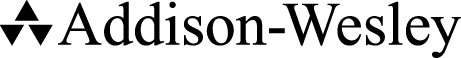
\includegraphics{AWlogoTitlePage-Mac}\\   % AW Mac
%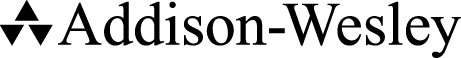
\includegraphics{AWlogoTitlePage_PC}  \\  %AW PC
{\footnotesize 
Boston~$\bullet$~Columbus~$\bullet$~Indianapolis~$\bullet$~New York~$\bullet$~San Francisco~$\bullet$~Amsterdam~$\bullet$~Cape Town\\[1ex]
Dubai~$\bullet$~London~$\bullet$~Madrid~$\bullet$~Milan~$\bullet$~Munich~$\bullet$~Paris~$\bullet$~Montreal~$\bullet$~Toronto~$\bullet$~Delhi~$\bullet$~Mexico City\\[1ex]
Sao Paulo~$\bullet$~Sidney~$\bullet$~Hong Kong~$\bullet$~Seoul~$\bullet$~Singapore~$\bullet$~Taipei~$\bullet$~Tokyo\\[1ex]
}
\end{center}
                               % The title page
\thispagestyle{empty}
\vspace*{\fill}
{\footnotesize 
\noindent Many of the designations used by manufacturers and sellers to distinguish their products are claimed as trademarks. Where those designations appear in this book, and the publisher was aware of a trademark claim, the designations have been printed with initial capital letters or in all capitals.\\
\hspace{\fill}\\
\noindent The author and publisher have taken care in the preparation of this book, but make no expressed or implied warranty of any kind and assume no responsibility for errors or omissions. No liability is assumed for incidental or consequential damages in connection with or arising out of the use of the information or programs contained herein.\\   % change to authors (plural) if this book has multiple authors
\hspace{\fill}\\
\noindent For information about buying this title in bulk quantities, or for special sales opportunities (which may include electronic versions; custom cover designs; and content particular to your business, training goals, marketing focus, or branding interests), please contact our corporate sales department at \mbox{corpsales}\linebreak[3]@\linebreak[3]pearsoned\linebreak[3].com or (800) 382-3419.\\
\hspace{\fill}\\
\noindent For government sales inquiries, please contact governmentsales@pearsoned.com.\\
\hspace{\fill}\\
\noindent For questions about sales outside the United States, please contact international@pearsoned.com.\\
\hspace{\fill}\\
\noindent Visit us on the Web: informit.com/aw\\     % use this line if you are publishing with AW
%\noindent Visit us on the Web: informit.com/ph\\   % use this line if you are publishing with PH
\hspace{\fill}\\
\noindent\textit{Library of Congress Cataloging-in-Publication Data}\\[.75ex]  % update this with info provided by your production editor
\textbf{LIBRARY OF CONGRESS CIP DATA WILL GO HERE; MUST BE ALIGNED AS INDICATED BY LOC}\\[.75ex]
\noindent Copyright~\copyright~2016 Pearson Education, Inc.\\
\hspace{\fill}\\
\noindent All rights reserved. Printed in the United States of America. This publication is protected by copyright, and permission must be obtained from the publisher prior to any prohibited reproduction, storage in a retrieval system, or transmission in any form or by any means, electronic, mechanical, photocopying, recording, or likewise. For information regarding permissions, request forms and the appropriate contacts within the Pearson Education Global Rights \& Permissions Department, please visit www.pearsoned.com/permissions/.\\[.75ex]

\noindent ISBN-13: {{isbn_13}}\\[-.5ex] % update this with info provided by your production editor 
\noindent ISBN-10: {{isbn_10}} \\[-.5ex] % update this with info provided by your production editor
\noindent Text printed in the United States on recycled paper at {{printer_info}}.\\[-.5ex] % update this with info provided by your production editor
\noindent First printing, {{first_printing}} % update this with info provided by your production editor
}
                                % The cataloging-in-publication page
\thispagestyle{empty}
\begin{center}For Theresa,\\ 
my one true love.
\end{center}
                      % The dedication page
\cleardoublepage
\parskip .5ex                       % Add space between Contents items
\tableofcontents                  % Make the Table of Contents 
\cleardoublepage                
\parskip 0in                         % Reset to zero interpar spacing
\cleardoublepage
\chapter*{Foreword}

The text of the foreword will go here.                 % Add foreword
\cleardoublepage
\chapter*{Preface}

The text of the preface will go here.  All the elements and commands offered within the text will work here as well.
                 % Add preface 
\include{ack}                        % Add acknowledgements 
\cleardoublepage
\chapter*{About the Author}

 % wrapfig doesn't like to be immediately after a chapter/section command 
 % so we are tricking it a bit with the \hspace and the \par commands.
\hspace*{\fill}\\  
\par\begin{wrapfigure}[12]{L}[0pt]{0pt}
\includegraphics[width=4cm]{AuthorPhoto}\end{wrapfigure}\noindent AUTHOR BIO WILL APPEAR HERE.  Lorem ipsum dolor sit amet, consectetur adipisicing elit, sed do eiusmod tempor incididunt ut labore et dolore magna aliqua. Ut enim ad minim veniam, quis nostrud exercitation ullamco laboris nisi ut aliquip ex ea commodo consequat. Duis aute irure dolor in reprehenderit in voluptate velit esse cillum dolore eu fugiat nulla pariatur. Excepteur sint occaecat cupidatat non proident, sunt in culpa qui officia deserunt mollit anim id est laborum. Lorem ipsum dolor sit amet, consectetur adipisicing elit, sed do eiusmod tempor incididunt ut labore et dolore magna aliqua. Ut enim ad minim veniam, quis nostrud exercitation ullamco laboris nisi ut aliquip ex ea commodo consequat. Lorem ipsum dolor sit amet, consectetur adipisicing elit, sed do eiusmod tempor incididunt ut labore et dolore magna aliqua. Ut enim ad minim veniam, quis nostrud exercitation ullamco laboris nisi ut aliquip ex ea commodo consequat. 
                   % Add about the author page
\cleardoublepage                  
%%%%%%%The front matter ends


%%%%%%%%%% Now we'll start on the main text for the book.  
%% Main Text:
\pagenumbering{arabic}		  % Arabic numbering
\include{chap1}  % Chapter 1
%% \include{glossary}        % Glossary 
%% %  just adding extra chapters for testing the TOC
%% \include{samplechap2}  % Chapter 2
%% \include{glossary}        % Glossary 
%% \include{samplechap3}  % Chapter 3
%% \include{glossary}        % Glossary 
%% \include{part2}            % Part II
%% \include{samplechap4}  % Chapter 4
%% \include{glossary}        % Glossary 
%% \include{samplechap5}  % Chapter 5
%% \include{glossary}        % Glossary 
%% \include{samplechap6}  % Chapter 6
%% \include{glossary}        % Glossary 
%% \include{samplechap7}  % Chapter 7
%% \include{glossary}        % Glossary 
%% \include{part3}            % Part III
%% \include{samplechap8}  % Chapter 8
%% \include{glossary}        % Glossary 
%% \include{samplechap9}  % Chapter 9
%% \include{glossary}        % Glossary 
%% \include{samplechap10}  % Chapter 10
%% \include{glossary}        % Glossary 

% Repeat this command for each part, chapter, or glossary file.
%
%%%%% End main text


%%%%%%%%%% Back matter starts
%
% If your book contains appendices, you will need to add those here. 
%\appendix               % Change to appendix numbering 
%\include{AppA}      % And add this line for each appendix file
%\include{AppB}

\cleardoublepage
\bibliographystyle{ieeetr-hacked}  % Your production editor and copy editor may want you to
                                                          % use a different bibliography style file. 
                                                          % You can input that style file here.  
\bibliography{samplebib}  % Loading the bibliography file.  
\nocite{*}  % \nocite is used because no citations appear in this sample text

\cleardoublepage
\include{index}  % If your book will include an index created outside of LaTeX, you'll likely receive a .rtf file, and you'll need to manually alter it to LaTeX, like this sample. 
% \printindex   % If your book will include a LaTeX-generated index, you'll include it with this line. 
%
%%%%%%% Back matter ends

\end{document}
